\documentclass[t]{beamer}
\usetheme[darktitle, framenumber, totalframenumber]{UniversityOfManchester}
\usepackage{sourcesanspro}

\usepackage{adjustbox}

\title{Real-time brain modelling with~SpiNNaker}
\subtitle{2015 Research Symposium}
\author{Andrew Mundy}

% Drawing
\usepackage{tikz}
\tikzstyle{every picture}+=[remember picture]
\tikzstyle{na}=[baseline=-.5ex]
\usetikzlibrary{arrows.meta, decorations.pathmorphing, positioning, shapes, topaths}
\tikzset{
  neuron/.style = {draw, very thick, fill=uomgrey, circle, text width=5pt,
                   text height=5pt, inner sep=0pt},
  box/.style = {draw, very thick},
  core/.style = {inner sep=10pt},
  core border/.style = {draw=black!15!white, line width=5pt},
  link/.style = {very thick, arrows={-Triangle[]}, shorten >=1pt},
  packet/.style = {ultra thick, draw, text height=10pt, text width=10pt,
                   inner sep=0pt},
  causal/.style = {line width=2.5pt, uompurple, shorten >=2pt,
                   arrows={-Triangle[]}},
}
%% Diagram to illustrate the algorithm
\usetikzlibrary{arrows.meta, bending, decorations.pathreplacing, positioning, shapes}

\tikzstyle{every picture}+=[remember picture]
\tikzset{
    neuron/.style = {
      fill=gray, circle, text width=5pt, text height=5pt, inner sep=0,
      draw=black!65!white, ultra thick,
    },
    box/.style = {
      ultra thick, color=black!70!white, draw,
    },
    ringbuffer/.style = {
      box, circle, text width=7.5pt, text height=7.5pt, inner sep=0,
    },
    matrix line/.style = {very thick, draw=black!50!white},
    relation/.style = {line width=2.5pt, black!45!white, arrows={Triangle[]-Triangle[]}},
    core/.style = {line width=4pt, draw=black!10!white, inner sep=10pt},
    link/.style = {ultra thick, black!80!white, arrows={-Triangle[]}, shorten >= 2pt},
    brace/.style = {decoration={brace, amplitude=5pt}, decorate, very thick},
    brace label/.style = {midway, align=center},
    brace label above/.style = {brace label, above=5pt},
    brace label below/.style = {brace label, below=5pt},
    value packet split/.style = {very thick, black!50!white},
    packet/.style = {above=2.5pt, text height=5pt, inner sep=0, value packet split, draw},
    spike packet/.style = {packet, text width=5pt},
    value packet/.style = {packet, text width=10pt},
}

\newcommand{\drawmatrix}[3]{%
  \draw [matrix line] (#1) rectangle ++(10pt * #2, -10pt * #3);
  \foreach \i in {2,...,#2}{%
    \draw [matrix line] ([xshift=10pt * \i - 10pt] #1) -- ++(0pt, -10pt * #3);
  }
  \foreach \j in {2,...,#3}{%
    \draw [matrix line] ([yshift=-10pt * \j + 10pt] #1) -- ++(10pt * #2, 0pt);
  }
}

\newcommand{\valuecore}[4]{%
  %% Draw a value-based transmission core:
  %% Arguments:
  %%    1. Name prefix
  %%    2. Number of neurons
  %%    3. Number of encoder dimensions
  %%    4. Number of decoder dimensions
  \begin{tikzpicture}
    %% Draw the filter and the encoder matrix
    \node [box, minimum width=40pt, minimum height=30pt]
         (#1_filter) {$H[z]$};
    \node [box, minimum height=#2*20pt + 5pt, minimum width=#3*10pt + 10pt,
           right=30pt of #1_filter.east] (#1_encoder) {
             \begin{tikzpicture}
               \drawmatrix{0pt, 0pt}{#3}{#2}
             \end{tikzpicture}
           };

    %% Connect them together
    \draw [link] (#1_filter) -- (#1_encoder);

    %% Draw the neurons
    \foreach \n in {1,...,#2}{%
      \node [right=25pt of #1_encoder.south east, neuron, yshift=\n*20pt - 7.5pt]
            (#1_\n) {};
      \draw [link] (#1_encoder.east |- #1_\n) -- (#1_\n);
    }

    % Draw the decoder
    \node [box, right=55pt of #1_encoder.east, minimum width=#4*10pt + 10pt,
           minimum height=#2*20pt + 5pt] (#1_decoder) {
            \begin{tikzpicture}
               \drawmatrix{0pt, 0pt}{#4}{#2}
            \end{tikzpicture}
           };

    %% Connect the neurons to the decoder
    \foreach \n in {1,...,#2}{%
      \draw [link] (#1_\n) -- (#1_\n -| #1_decoder.west);
    }
  \end{tikzpicture}
}

\newcommand{\spikescore}[3]{%
  %% Draw a value-based transmission core:
  %% Arguments:
  %%    1. Name prefix
  %%    2. Number of neurons
  %%    3. Number of pre-synaptic neurons
  \begin{tikzpicture}
    %% Draw the filter and the encoder matrix
    \node [box, minimum height=#2*20pt + 5pt, minimum width=#2*10pt + 10pt]
          (#1_weights) {
             \begin{tikzpicture}
               \drawmatrix{0pt, 0pt}{#2}{#3}
             \end{tikzpicture}
           };

    %% The multiplex which takes spikes and produces packets.
    \node [trapezium, box, rotate=-90,
           minimum width=20pt * #2, minimum height=15pt,
           trapezium stretches, trapezium angle=75,
           right=117.5pt of #1_weights.east, anchor=south] (#1_mux) {};

    %% Draw the ring buffers and the neurons
    \foreach \n in {1,...,#2}{%
      \node [right=30pt of #1_weights.south east, ringbuffer, yshift=\n*20pt - 7.5pt]
            (#1_ringbuffer_\n) {};
      \node [right=30pt of #1_ringbuffer_\n, neuron] (#1_\n) {};

      \draw [link] (#1_weights.east |- #1_ringbuffer_\n) -- (#1_ringbuffer_\n);
      \draw [link] (#1_ringbuffer_\n) -- (#1_\n);
      \draw [link] (#1_\n) -- (#1_\n -| #1_mux.south);

      \draw [box, very thick, arrows={-Straight Barb[bend, width=3pt, length=3pt]}]
        (#1_ringbuffer_\n.center)++(-45:10pt)
        arc [start angle=-45, delta angle=-90, x radius=10pt, y radius=10pt];
      \draw [box] (#1_ringbuffer_\n.north west) -- (#1_ringbuffer_\n.south east);
      \draw [box] (#1_ringbuffer_\n.south west) -- (#1_ringbuffer_\n.north east);
    }
  \end{tikzpicture}
}

\newcommand{\valueexample}{%
  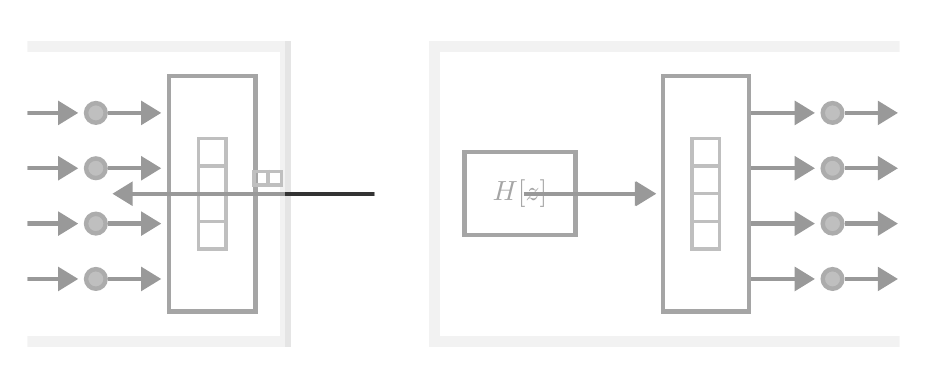
\begin{tikzpicture}[na]
    % Clip all the following drawing by this rectangle
    \clip (13pt, -60pt) rectangle ++(315pt, 120pt);

    %% Create the two cores and connect them
    \node [core] (A) {\valuecore{A}{4}{1}{1}};
    \node [core, right=50pt of A] (B) {\valuecore{B}{4}{1}{1}};
    \draw [link] (A_decoder) -- (B_filter)
      node [pos=.4, value packet] (val1) {};
    \draw [value packet split] (val1.north) -- (val1.south);

    %% Draw extra input and output connections
    \draw [link] ([xshift=-50pt] A_filter.west) -- (A_filter.west);
    \draw [link] (B_decoder.east) -- ++(50pt, 0);

    %% Hide the earlier part of A and the latter part of B
    \fill [fill opacity=0.5, white]
    ([xshift=-2.5pt] A_4.west |- A.north west) rectangle ([xshift=-50pt] A.south west);
    \fill [fill opacity=0.5, white]
      (B_4.east |- B.north east) rectangle ([xshift=50pt] B.south east);
  \end{tikzpicture}
}

\newcommand{\spikeexample}{%
  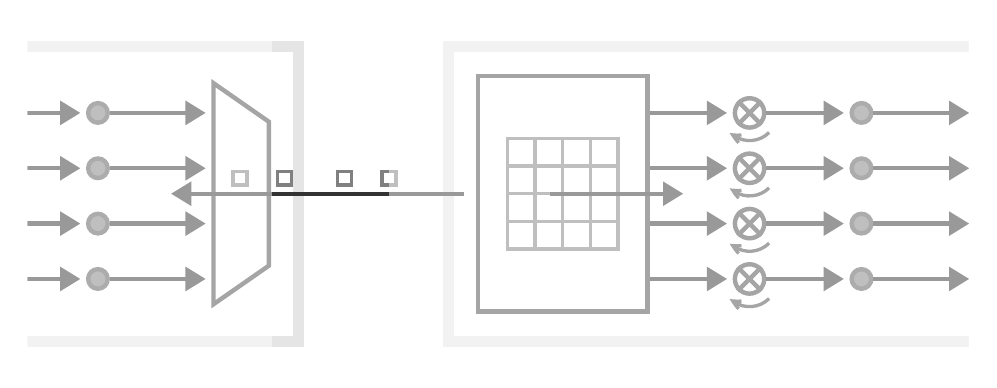
\begin{tikzpicture}[na]
    % Clip all the following drawing by this rectangle
    \clip (13pt, -60pt) rectangle ++(340pt, 120pt);

    %% Create the two cores and connect them, mark spike packets should be placed
    \node [core] (A) {\spikescore{A}{4}{3}};
    \node [core, right=50pt of A] (B) {\spikescore{B}{4}{4}};
    \draw [link] (A_mux.north) -- (B_weights)
      node [pos=0.25, spike packet] (sp1) {}
      node [pos=0.40, spike packet] (sp2) {}
      node [pos=0.60, spike packet] (sp3) {}
      node [pos=0.75, spike packet] (sp4) {};

    %% Draw extra input and output connections
    \draw [link] ([xshift=-50pt] A_weights.west) -- (A_weights.west);
    \draw [link] (B_mux.north) -- ++(50pt, 0);

    %% Hide the earlier part of A and the latter part of B
    \fill [fill opacity=0.5, white]
    ([xshift=-2.5pt] A_4.west |- A.north west) rectangle ([xshift=-50pt] A.south west);
    \fill [fill opacity=0.5, white]
      (B_4.east |- B.north east) rectangle ([xshift=50pt] B.south east);
  \end{tikzpicture}
}


\usepackage{siunitx}

\begin{document}

\maketitle

\begin{frame}{How to build a brain?}
  % Hypothesis -> Predictions (computational experiments) -> Test hypothesis
  %  - Computational experiments are expensive
  %  - SpiNNaker *should* make this cheaper...
  \begin{columns}[T]
    \begin{column}{.55\textwidth}
      \begin{tikzpicture}
        \node at (90:30pt) [anchor=south] (hypothesis) {
          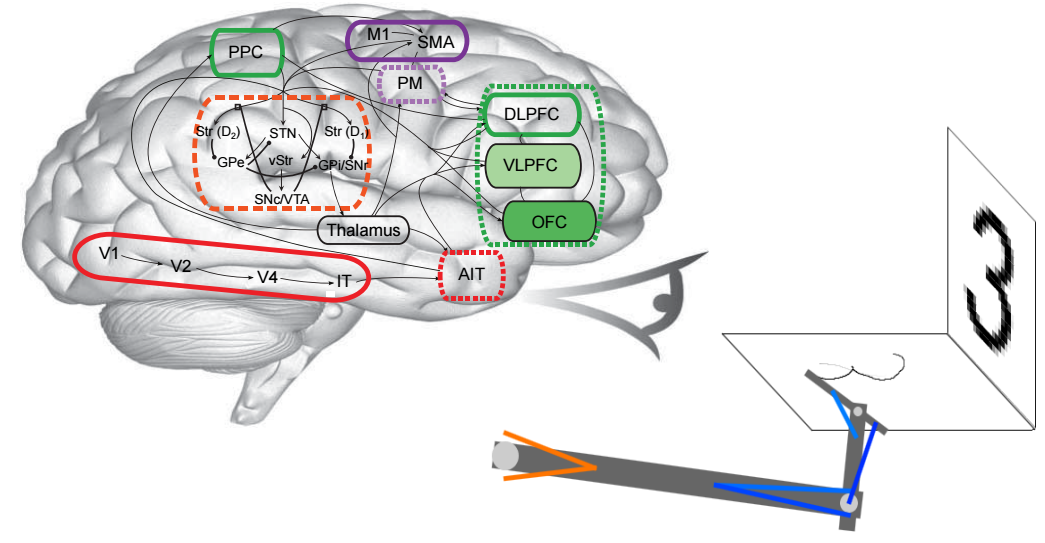
\includegraphics[width=140pt]{figures/spaun}
        };
        \node at (90-120:30pt) [anchor=north west] (simulation) {
          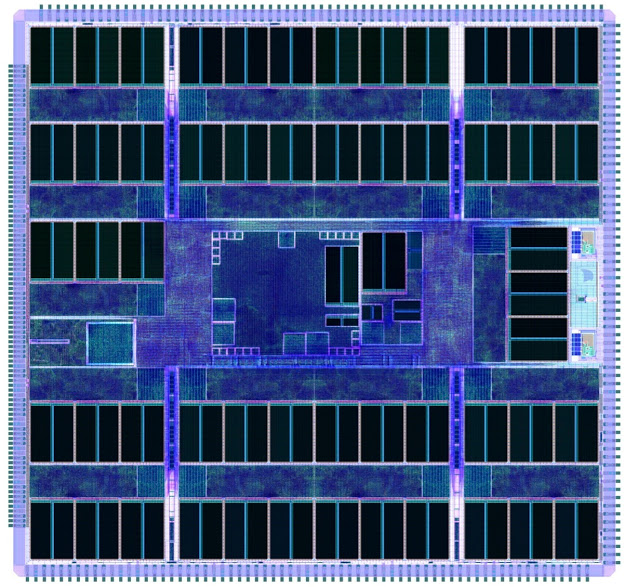
\includegraphics[width=60pt]{figures/spinnaker}
        };
        \node at (90-240:30pt) [anchor=north east] (comparator) {
          Biology
        };
      \end{tikzpicture}
    \end{column}
    \begin{column}{.44\textwidth}
      \textbf{Spaun}
      \begin{itemize}
        \item \num{2.5}~M neurons
        \item \SI{2.5}{\hour} per second of simulation
      \end{itemize}

      \textbf{SpiNNaker} \textit{should} reduce this cost...
      \begin{itemize}
        \item Larger models
        \item Real-world interaction
      \end{itemize}
    \end{column}
  \end{columns}

  % Add some labels, linking the items together
  \begin{tikzpicture}[overlay]
    \begin{scope}[uompurple, line width=3pt, arrows={-Triangle[]}, bend left]
      \draw (hypothesis) to (simulation);
      \draw (simulation) to (comparator);
      \draw (comparator) to (hypothesis.south);
    \end{scope}
  \end{tikzpicture}
\end{frame}

\begin{frame}{How to simulate a brain?}
  % Explain type of neural model
  %  - Point spiking neurons
  %  - Connection weight matrix + synaptic dynamics
  % Exploit parallelism: map neural models onto SpiNNaker
  \centering
  \vfill
  \begin{tikzpicture}
  % Draw the neuron model
  \node (neuron-model) {
    \begin{tikzpicture}
      % Draw the pre-neurons
      \node (pre-neurons) {
        \begin{tikzpicture}
          \foreach \n in {1,...,4}{
            \draw (0, \n*15pt) node [neuron] (pre-\n) {};
          }
        \end{tikzpicture}
      };

      % Draw the post-neurons
      \node (post-neurons) [right=150pt of pre-neurons] {
        
\begin{tikzpicture}
          \foreach \n in {1,...,4}{
            \draw (0, \n*15pt) node [neuron] (post-\n) {};
          }
        \end{tikzpicture}
      };

      % Draw the connectivity matrix
      \foreach \x in {1,...,4}{%
        \foreach \y in {1,...,4}{%
          \draw [very thick, arrows={-Triangle[]}, shorten >=4pt]
                (pre-\x) to (post-\y);
        }
      }
    \end{tikzpicture}
  };

  % Draw a simplified representation of SpiNNaker
  \node (spinnaker) [below=10pt of neuron-model.south] {
    
\begin{tikzpicture}
      % Only draw two cores
      \begin{scope}[minimum width=40pt, minimum height=40pt]
        \node (core0) [core border] {};
        \node (core1) [core border, right=80pt of core0] {};
      \end{scope}

      % Add some links
      \foreach \c in {0, 1}{
        \draw [core border] (core\c.north) -- ++(0, 10pt);
        \draw [core border, line cap=rect]
          (core\c.north east) -- ++(5pt, 5pt);
        \draw [core border] (core\c.south) -- ++(0, -10pt);
        \draw [core border, line cap=rect]
          (core\c.south west) -- ++(-5pt, -5pt);
      }
      \draw [core border] (core0.west) -- ++(-10pt, 0);
      \draw [core border] (core1.east) -- ++(10pt, 0);
      \draw [core border] (core0.east) -- (core1.west)
        node [midway, coordinate] (network) {};
    \end{tikzpicture}
  };

  % Show the mapping processing
  % Neurons to processing cores
  \onslide<2-> {
    % Population 0 to core 0
    \draw [rounded corners, line width=5pt, uompurple]
          (pre-neurons.south west) rectangle (pre-neurons.north east);
    \draw [line width=2.5pt, uompurple, arrows={-Triangle[]}] (pre-neurons.south) to (core0);
  }
  \onslide<3-> {
    % Population 1 to core 1
    \draw [rounded corners, line width=5pt, uompurple]
          (post-neurons.south west) rectangle (post-neurons.north east);
    \draw [line width=2.5pt, uompurple, arrows={-Triangle[]}] (post-neurons.south) to (core1);
  }

  % Connectivity to routing
  \onslide<4-> {
    \path (pre-neurons) -- (post-neurons) node [midway, coordinate] (mid_conn) {};
    \node at (mid_conn) [line width=5pt, draw, circle, uomyellow,
                         minimum height=60pt, minimum width=60pt] (highlight conn) {};
  }
  \onslide<5-> {
    \draw [line width=2.5pt, uomyellow, arrows={-Triangle[]}, shorten >=3pt]
      (highlight conn) to (network);
  }

  % Connectivity to weight matrix
  \onslide<6-> {
    \draw [line width=2.5pt, uomyellow, arrows={-Triangle[]}]
      (highlight conn) to (core1);
  }
\end{tikzpicture}

  \vfill
\end{frame}

\begin{frame}{How to simulate a neural net?}
  % Neural processing on SpiNNaker: how to
  \begin{minipage}{1.2\textwidth}
    \centering
    \hspace{-5.2em}
    \begin{adjustbox}{scale=.9}
      \spikeexample
    \end{adjustbox}
  \end{minipage}

  \vskip\baselineskip

  % Step by step operation
  \only<2>{\large
    \tikz[na] \node [coordinate] (n0) {};%
    Simulate neurons\\
    Send ``spike'' packets over the network%
      \tikz[na] \node [coordinate] (p0) {};
  }
  \only<3>{\large
    Receive ``spike'' packets, \tikz[na] \node [coordinate] (r0) {};\\
    look up synaptic weights \tikz[na] \node [coordinate] (r1) {};
  }
  \only<4>{\large
    Insert weights into ring buffers%
    \tikz[na] \node [coordinate] (i0) {};
  }

  % Progressively add labels to this diagram
  \begin{tikzpicture}[overlay, arrows={-Triangle[]}, shorten >=2pt,
                      shorten <= 2pt, ultra thick, uompurple, na]
    % Neuron update
    \draw<2> [out=180, in=-135] (n0.center) to (A_1.south west);
    \draw<2> [out=45, in=-45, shorten >=6pt] (p0.center) to (sp2);

    % Receive spike packets
    \draw <3> [shorten >= 0, out=60, in=-105] (r0.center) to
      ([xshift=-.25em, yshift=-.5em] sp4.south);
    \draw <3> [shorten >= 0, out=25, in=-105] (r1.center) to
      ([xshift=-15pt, yshift=20pt] B_weights.south);

    % Insert into ring buffers
    \draw <4> [out=0, in=265] (i0) to
      ([xshift=-2em, yshift=-.5em] B_ringbuffer_1);
  \end{tikzpicture}
\end{frame}

% Constraints model - show how the NEF makes this very hard
\begin{frame}{Not so easy\ldots}
  \begin{columns}[c]
    \begin{column}{.35\textwidth}%
      % Stack diagram indicating constraints
      \begin{tikzpicture}
  % Clip all the following drawing by this rectangle
  \clip (13pt, -25pt) rectangle ++(140pt, 160pt);

  % Processing cores
  \begin{scope}[core border, text width=30pt, text height=30pt]
    \node (0, 0) [anchor=south west, draw] (core1) {};
    \node [draw, right=40pt of core1] (core2) {};
  \end{scope}

  % DTCMs
  \begin{scope}[core border, text width=60pt, text height=20pt]
    \foreach \n in {1, 2}
    {
      \node [draw, above=20pt of core\n] (dtcm\n)
      {
      };
    }
    \path (dtcm1) -- (dtcm2) node [midway] (middtcm) {};
  \end{scope}

  % SDRAM
  \node [core border, text width=160pt, text height=40pt,
         above=20pt of middtcm] (sdram) {};

  % Draw synaptic weight matrices in SDRAM and synaptic rows in DTCM
  \foreach \n/\w in {1/5, 2/7}
  {
    \node [above=25pt of dtcm\n]
    {
      \begin{tikzpicture}
        \draw [very thick, step=7.5pt] (0, 0) grid ++(\w*7.5pt, 12*7.5pt);
      \end{tikzpicture}
    };

    \node at (dtcm\n)
    {
      \begin{tikzpicture}
        \draw [very thick, step=7.5pt] (0, 0) grid ++(\w*7.5pt, 7.5pt);
      \end{tikzpicture}
    };
  }

  % Draw links between elements in the memory hierarchy
  \foreach \n in {1, 2}
  {
    \draw [line width=7.5pt] (core\n.north) -- (dtcm\n.south);
    \draw [line width=1.5pt] (dtcm\n.north) -- (dtcm\n.north |- sdram.south)
      node [midway, coordinate] (sdramlink\n) {};
  }

  % Network fabric
  \draw [line width=1pt, arrows={-Triangle[]}]
    (core1.south) |- ([xshift=40pt, yshift=-20pt] core2.south);
  \draw [line width=1pt] (core2.south) -- ++(0, -20pt);
  \draw [line width=1pt] ([yshift=-20pt] core1.south) -- ++(-15pt, 0);
\end{tikzpicture}

    \end{column}\hfill
    \begin{column}{.62\textwidth}
      \begin{itemize}
        \item \tikz[na]\node [coordinate] (n0) {};Limited SDRAM access bandwidth
        \item \tikz[na]\node [coordinate] (n1) {};DTCM small
        \item \tikz[na]\node [coordinate] (n2) {};Real-time constraints
        \item \tikz[na]\node [coordinate] (n3) {};Network utilisation
      \end{itemize}

      \onslide<6>{\textbf{NEF is not a good fit for SpiNNaker as designed\ldots}}
      \begin{itemize}
        \item<6> Dense weight matrices
        \item<6> High firing rates
      \end{itemize}
    \end{column}
  \end{columns}

  % Progressively add labels to this diagram to indicate what the constraints
  % are.
  \begin{tikzpicture}[overlay, arrows={-Triangle[]}, shorten >=2pt,
                      shorten <= 5pt, ultra thick, uompurple]
    % SDRAM access
    \draw<2> [out=180, in=45] ([xshift=-2ex] n0) to (sdramlink2);
    \draw<3> [out=180, in=0] ([xshift=-2ex] n1) to (dtcm2.east);
    \draw<4> [out=180, in=45] ([xshift=-2ex] n2) to (core2.east);
    \draw<5> [out=180, in=45] ([xshift=-2ex] n3) to
                              ([xshift=20pt, yshift=-15pt] core2.south);
  \end{tikzpicture}
\end{frame}

\begin{frame}{\ldots use factored weight matrices}
  % Diagram to show factoring of the weight matrix
  \centering
  \vfill
  {\Large Useful property of the NEF:}
  \vfill
  \begin{tikzpicture}
    \node (unfactored) [label=below:Weight matrix] {
      \begin{tikzpicture}
        \drawmatrix{0, 0}{4}{4};
      \end{tikzpicture}
    };

    \node [right=of unfactored] (equals) {$\equiv$};

    \node (encoder) [right=of equals, label=below:Encoder] {
      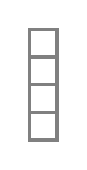
\begin{tikzpicture}
        \drawmatrix{0, 0}{1}{4};
      \end{tikzpicture}
    };

    \node [right=of encoder] (times) {$\times$};

    \node (decoder) [right=of times, label=below:Decoder] {
      
\begin{tikzpicture}
        \drawmatrix{0, 0}{4}{1};
      \end{tikzpicture}
    };
  \end{tikzpicture}
  \vfill
\end{frame}

\begin{frame}{Change the algorithm\ldots}
  % Weight matrix can be factored

  % Changes to the algorithm
  \begin{minipage}{1.2\textwidth}
    \centering
    \hspace{-5.2em}
    \begin{adjustbox}{scale=.9}
      \valueexample
    \end{adjustbox}
  \end{minipage}

  \vskip\baselineskip

  {\large
    \only<2>{
      \tikz[na] \node [coordinate] (n0) {};%
      Simulate neurons \\
      Multiply spikes by the ``decoder'' matrix \tikz[na] \node [coordinate] (n1) {};
    }
    \only<3>{
      Transmit each resulting component \tikz[na] \node [coordinate] (t0) {};
    }
    \only<4>{
      Apply the synaptic filter \tikz[na] \node [coordinate] (f0) {};
    }
    \only<5>{
      Multiply the vector by the ``encoder'' matrix \tikz[na] \node [coordinate] (e0) {};
    }
  }

  % Progressively add labels to this diagram
  \begin{tikzpicture}[overlay, arrows={-Triangle[]}, shorten >=2pt,
                      shorten <= 2pt, ultra thick, uompurple, na]
    % Neuron update
    \draw<2> [out=180, in=-135] (n0.center) to (A_1.south west);
    \draw<2> [out=45, in=-45, shorten >=6pt] (n1.center) to (A_decoder);

    % Transmit value packets
    \draw <3> [shorten >= 0, out=60, in=-60] (t0.center) to
      ([xshift=-1em, yshift=-1em] val1.south);

    % Receive and apply synaptic filter
    \draw <4> [shorten >= 0, out=0, in=-90] (f0.center) to
      ([xshift=-1em, yshift=-.5em] B_filter.south);

    % Encode to form neuron inputs
    \draw <5> [shorten >= 0, out=25, in=-60] (e0.center) to
      ([xshift=-1.5em, yshift=1em] B_encoder.south);
  \end{tikzpicture}
\end{frame}

% Constraints model - how do factored weight matrices make this better
\begin{frame}{The benefits\ldots}
  \begin{columns}[c]
    \begin{column}{.35\textwidth}%
      % Stack diagram indicating constraints
      \begin{tikzpicture}
  % Clip all the following drawing by this rectangle
  \clip (13pt, -25pt) rectangle ++(140pt, 160pt);

  % Processing cores
  \begin{scope}[core border, text width=30pt, text height=30pt]
    \node (0, 0) [anchor=south west, draw] (core1) {};
    \node [draw, right=40pt of core1] (core2) {};
  \end{scope}

  % DTCMs
  \begin{scope}[core border, text width=60pt, text height=20pt]
    \foreach \n in {1, 2}
    {
      \node [draw, above=20pt of core\n] (dtcm\n)
      {
      };
    }
    \path (dtcm1) -- (dtcm2) node [midway] (middtcm) {};
  \end{scope}

  % SDRAM
  \node [core border, text width=160pt, text height=40pt,
         above=20pt of middtcm] (sdram) {};

  % Draw synaptic weight matrices in SDRAM and synaptic rows in DTCM
  \foreach \n/\w in {1/5, 2/7}
  {
    \node [above=25pt of dtcm\n]
    {
      \begin{tikzpicture}
        \draw [very thick, step=7.5pt] (0, 0) grid ++(\w*7.5pt, 12*7.5pt);
      \end{tikzpicture}
    };

    \node at (dtcm\n)
    {
      \begin{tikzpicture}
        \draw [very thick, step=7.5pt] (0, 0) grid ++(\w*7.5pt, 7.5pt);
      \end{tikzpicture}
    };
  }

  % Draw links between elements in the memory hierarchy
  \foreach \n in {1, 2}
  {
    \draw [line width=7.5pt] (core\n.north) -- (dtcm\n.south);
    \draw [line width=1.5pt] (dtcm\n.north) -- (dtcm\n.north |- sdram.south)
      node [midway, coordinate] (sdramlink\n) {};
  }

  % Network fabric
  \draw [line width=1pt, arrows={-Triangle[]}]
    (core1.south) |- ([xshift=40pt, yshift=-20pt] core2.south);
  \draw [line width=1pt] (core2.south) -- ++(0, -20pt);
  \draw [line width=1pt] ([yshift=-20pt] core1.south) -- ++(-15pt, 0);
\end{tikzpicture}

    \end{column}\hfill
    \begin{column}{.62\textwidth}
      \begin{itemize}
        \item Significant memory savings
        \begin{itemize}
          \item<2-> Upwards of 90\%
        \end{itemize}
        \item Reduced compute
        \begin{itemize}
          \item<3-> $2\times$ neurons per core
        \end{itemize}
        \item Less network traffic
        \begin{itemize}
          \item<4-> Vector size $\ll$ number of neurons
        \end{itemize}
      \end{itemize}
    \end{column}
  \end{columns}
\end{frame}

\begin{darkframes}
  \begin{frame}{\hspace{1em}}
    \centering
    \vfill
    {\huge Demo}
    \vfill
  \end{frame}
\end{darkframes}

\begin{frame}{In conclusion\ldots}
  
\end{frame}

\begin{darkframes}
  \begin{frame}{\hspace{1em}}
    \centering
    \vfill
    {\huge Thank you}\\\vskip\baselineskip
    {\LARGE Any questions?}
    \vfill
  \end{frame}
\end{darkframes}
  
\end{document}
